\section{Computational Results}\label{sec:results}

The objective of our computational study is to assess whether LABD accelerates Benders decomposition while preserving solution quality, and whether learning-guided selection and dual prediction improve on a non-learning benchmark that also solves only part of the subproblems exactly. We conduct our experiments on the stochastic capacitated facility location problem (SCFLP), which determines facility openings and customer allocations under uncertain demand. Its formulation and further experimental details are given in Appendix~\ref{app:experiments}.

\paragraph{Experimental setting.} We compare Standard BD with LABD and with the random sampling and dual-averaging benchmark (RND) adapted from~\cite{bertsimas2024stochastic}. RND randomly selects subproblems for exact evaluation and transfers an averaged dual-feasible solution to the remaining subproblems; we implement its no-restart variant within the same single-tree framework. We vary the exact-subproblem share $p/|\mathcal M|$ across $5\%$, $15\%$ and $25\%$. LABD uses $|\mathcal K_0|=5$ warm-up iterations and three-dimensional representations constructed from warm-up dual trajectories. All methods are implemented within a single-tree multi-cut Benders framework, with cuts generated at LP-relaxation and integer-feasible callbacks, a three-hour time limit and a relative optimality tolerance of $0.1\%$. Each run uses 16 threads and 128\,GiB on two Intel Xeon 6972P processors (2.4\,GHz), with Python~3.11 and Gurobi~12.0.0.

\paragraph{Data.} We use SCFLP instances from the $p$-series of~\cite{holmberg1999exact}. Each deterministic instance is extended to a stochastic setting with $|\mathcal M|\in\{100,300,500\}$ scenarios for the sample average approximation. Scenario-dependent demands are generated following a procedure adapted from~\cite{bodur2017strengthened}, with scaling where necessary to ensure relatively complete recourse. The instances and the data generation are detailed in Appendix~\ref{app:instances}.

\paragraph{Performance metrics.} For each method $a$, let $\widehat{\mathbf x}_a$ denote its returned first-stage solution and $V_a:=V(\widehat{\mathbf x}_a)$ the full objective evaluated at this solution across all scenarios. Let $V_{\mathrm{BD}}$ denote the objective value of the matched Standard BD run, and $T_a$ and $T_{\mathrm{BD}}$ the respective runtimes; the final exact evaluation of $\widehat{\mathbf x}_a$, used only to compute $V_a$, is not included in $T_a$. We report
\begin{equation}\label{eq:metrics}
\Delta_a(\%):=100\,\frac{V_a-V_{\mathrm{BD}}}{|V_{\mathrm{BD}}|}\qquad\text{and}\qquad\tau_a:=\frac{T_a}{T_{\mathrm{BD}}}.
\end{equation}
If Standard BD reaches the time limit, $\Delta_a$ compares best feasible solutions (Appendix~\ref{app:conventions}); $\tau_a<1$ means faster than Standard BD.

\begin{figure}[t]
\centering
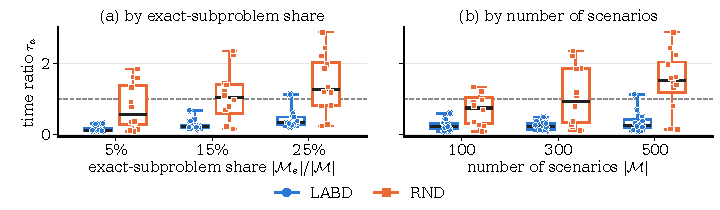
\includegraphics[width=\textwidth]{figures/fig_share.pdf}
\caption{Time ratio $\tau_a$ by exact-subproblem share (a) and by number of scenarios (b) for the configurations solved by Standard BD. The dashed line $\tau_a=1$ is Standard BD.}\label{fig:share}
\end{figure}



\begin{table}[!b]
\centering
\caption{Gap $\Delta_a$ (\%) relative to Standard BD on the configurations it solves (left) and on p20, where it reaches the time limit (right; over the configurations in which the method finds a feasible solution; negative is better). Opt.: $\Delta_a=0$; NS: no feasible solution.}\label{tab:gap}
\setlength{\tabcolsep}{5pt}
\begin{tabular}{lrrrr!{\vrule width 1pt}rrrr}
\toprule
& \multicolumn{4}{c!{\vrule width 1pt}}{\textbf{BD solved} ($n=36$)} & \multicolumn{4}{c}{\textbf{BD time limit} ($n=9$)}\\
\cmidrule(lr){2-5}\cmidrule(lr){6-9}
Method & Opt. & Mean & Med. & Max. & NS & Mean & Med. & Max.\\
\midrule
LABD & 34 & 0.08 & 0.00 & 1.56 & 0 & $-$1.86 & $-$2.35 & 2.38\\
RND  & 30 & 0.21 & 0.00 & 1.56 & 3 & 12.49 & 8.93 & 27.12\\
\bottomrule
\end{tabular}
\end{table}

\paragraph{Results.} Standard BD solves four of the five instances within the time limit for every number of scenarios, which gives 36 solved configurations per inexact method. Fig.~\ref{fig:share}(a) shows that LABD is markedly faster than Standard BD at every exact-subproblem share: it is about $4.6$ times faster in the median, and close to ten times faster when only $5\%$ of the subproblems are solved exactly. RND, which also solves only part of the subproblems exactly, gains much less: it is faster than Standard BD at the smallest share, close to it at $15\%$, and slower at $25\%$. The time ratio grows with the exact share, since each additional exact subproblem is solved in every cut-generation round, but for LABD this effort buys no better solutions: the smallest share already yields the optimal objective in almost every configuration. A small set of representative subproblems therefore carries most of the dual information needed to generate effective cuts, and the duals of the remaining subproblems can be inferred from it at negligible cost.

Fig.~\ref{fig:share}(b) shows how this advantage evolves with the size of the problem. As the number of scenarios grows from 100 to 500, the median time ratio of LABD remains between $0.21$ and $0.25$, whereas that of RND rises from $0.74$ to $1.53$. The benefit of LABD is thus maintained as the number of subproblems grows, while that of random selection vanishes.

Table~\ref{tab:gap} shows that the speed of LABD does not come at the expense of solution quality. LABD returns the optimal objective in 34 of the 36 solved configurations, against 30 for RND, and its mean gap is less than half that of RND. In the two configurations where LABD deviates, the gap remains below $1.6\%$.

The differences are sharper on p20, where Standard BD stops at the time limit with an optimality gap of $17$--$33\%$. LABD finds a feasible solution in all nine configurations and improves on the Standard BD incumbent in seven of them, by $1.86\%$ on average. RND returns no feasible solution in three configurations, because every integer candidate found during branch and bound was cut off by a violated Benders cut, and its solutions in the other six are on average $12.5\%$ worse than the Standard BD incumbent.

Since LABD and RND solve the same number of subproblems exactly, these differences reflect the representation-based selection and the certified prediction of LABD.
